\documentclass[lang=cn,newtx,10pt,scheme=chinese,bibend=bibtex,hang]{Maya}


\newcommand{\ccr}[1]{\makecell{{\color{#1}\rule{1cm}{1cm}}}}

\usepackage{tasks}
\settasks{
	label = \Alph*.,
	label-offset={0.4em},
	label-align = left,
	column-sep = {10pt},
	label-width = 2ex,
	item-indent = {40pt},
	before-skip = {-0.7em},
	after-skip ={-0.7em},
}
% \usepackage{graphicx}
\usepackage{caption}
\usepackage{enumerate}
\usepackage{pifont}
\usepackage{hyperref} 
\newcommand{\cmark}{\ding{51}} % 打勾符号
\newcommand{\xmark}{\ding{55}} % 打叉符号
\newcommand{\Tquestion}[1]{#1 \hfill\cmark}
\newcommand{\Fquestion}[1]{#1 \hfill\xmark}
\newcommand{\jiexi}[1]{{\color{myorange}\kaishu {\bf 解析:}{#1}}}
\newcommand{\daan}[2]{\vspace{0.25em}{\color{myorange}\kaishu {\bf 答案:}{#1} \hspace{0.5em} {#2} }}
\newcommand{\choosenum}{1}
\begin{document}
\subtitle{低压电工证部分错题}
%%% Command2是document之后的配置
\makecover
\clearpage
\pagenumbering{roman} % 设置页码为阿拉伯数字
\setcounter{page}{1} % 在这里重置页码
\tableofcontents
\clearpage
\pagenumbering{arabic} % 设置页码为阿拉伯数字
\setcounter{page}{1} % 在这里重置页码

\setlength{\parindent}{2em}   %首行缩进失效了

























%%%%%%%%%%%%%%%%%%%%%%%%%%%%%%%%%%%%%%%%%%%%%%%%%%%%%%%%%%%%%%%%%%%%%%%%%%%%%%%%%%%%%%%%%%%%% 正文

    \chapter{准备阶段(Preamble)}

\section{Intend}
The practice describes the pattern for specifying requirements.

这个文档描述了具有需求。

\subsection{Motivation/Pros}
\begin{enumerate}
	\item Reduction of language effects (misunderstandings);
	\item Supports unambiguousness of syntax;
	\item Supports creation of high quality requirements;
	\item Support time-efficient creation of requirements.
\end{enumerate}
中文解释
\begin{enumerate}[label=\textbullet]
	\item  减少语言影响(误解);
	\item  支持语法的明确性;
	\item  支持高质量需求的创建;
	\item  支持高效的需求创建。
\end{enumerate}

\subsection{Reference(主要参考文档)}

	\begin{enumerate}[label=\alph*.]
		\item   SAEJ1772.pdf\cite{SAE} $\bigstar \bigstar \bigstar$
		\item   Practice\_Requirement\_Pattern.pdf\cite{Pattern}
		\item 	Review\_protocol\_Template.xlsm\cite{Review}
		\item 	C001-PHEV项目BOBCDCD变换器总成软件规格书\cite{PHEV}
		\item   GB-T18487.1-2015.pdf\cite{GB18487} $\bigstar \bigstar \bigstar$
		\item   国内外电动汽车充电系统标准综述\cite{zs}
		\item   10kW电动汽车车载充电机及其软件策略研究\_赵春洋.pdf\cite{zhao}
		\item 	IEC61851-1-2010-控制导引电路相关内容\cite{IEC61851} $\bigstar \bigstar \bigstar$
	\end{enumerate}
 
\newpage
\section{Elements of a Requirement}
	本小节描述了软件需求规范;

	\begin{table}[h]
		\renewcommand{\arraystretch}{1.3}
		\centering
		\caption{Elements of a Requirement}
		\begin{tabular}{|p{2.5cm}|p{2cm}|p{6cm}|}  
			\specialrule{0.2em}{0pt}{0pt} 
			\centering \cellcolor{mygray} \textbf{Element}  & \multicolumn{2}{l|}{\cellcolor{mygray} \textbf{Description}}  \\    
			\hline
			\textcolor{winered}{<event/condition>}  & \multicolumn{2}{p{8cm}|}{The event that shall trigger the \textcolor{mygreen1}{<action>} when it occurs. \newline OR: The condition that shall be fulfilled to conduct the \textcolor{mygreen1}{<action>}} \\
			\hline
			\textcolor{mybule}{<actor>}  & \multicolumn{2}{p{8cm}|}{The acting part, i.e. the one who is obliged to evaluate the \textcolor{winered}{<event/condition>} and conduct \textcolor{mygreen1}{<action>}} \\
			\hline
			\textcolor{mypurple}{<legal binding>}   &  \multicolumn{2}{p{8cm}|}{Key word signifying the relevance of the requirement. Following key words are applicable (in accordance to RFC 2119)} \\
			\cline{2-3}
						&shall       & This word mean that the item is an absolute requirement. \\
						&shall not   & This phrase mean that the item is an absolute prohibition.\\
						&should      &This word mean that there may exist valid reasons to ignore
						the item, but the full implications must be understood and
						carefully weighed before choosing a different course.\\
						&should not           &This phrase mean that there may exist valid reasons
						when the item is acceptable or even useful, but the full
						implications should be understood and the case carefully
						weighed before implementing any behavior described with
						this label.\\
						&may          &This word mean that the item is truly optional.\\
						&will, is           &These keywords identify a statement of fact, not a
						requirement.\\
			\cline{2-3}
						&    \multicolumn{2}{p{8cm}|}{For objects of type “Req-XXX” only keywords “shall” and “shall not” shall
						be used.\newline
						For objects of type other than “Req-XXX”, like “Heading” or
						“Information” only keywords “should”, “should not”, “may”, “will”, and
						“is” shall be used.}\\
			\hline 
			\textcolor{mygreen1}{<action>}& \multicolumn{2}{p{8cm}|}{The actions being conducted by \textcolor{mybule}{<actor>} when the \textcolor{winered}{<event>} occurs or the
			\textcolor{winered}{<condition>} is fulfilled.}\\
			\hline
			\textcolor{mygreen2}{<object of action>} & \multicolumn{2}{p{8cm}|}{Optional specification of the object that undergoes the \textcolor{mygreen1}{<action>}.}\\
			\specialrule{0.2em}{0 pt}{0pt} 
		\end{tabular}
	\end{table}


\subsection{Requirements Pattern}

\subsubsection*{Case1}
	\begin{mybox}
		\centering
		\textcolor{mybule}{<actor>}  \textcolor{mypurple}{<legal binding>} \textcolor{mygreen1}{<action>} \textcolor{mygreen2}{<object of action>}\textcolor{winered}{<event/condition>}
	\end{mybox}
	\begin{enumerate}
		\item \textcolor{mybule}{The system} \textcolor{mypurple}{shall} \textcolor{mygreen1}{turn on} \textcolor{winered}{when the power button is pressed while the system is off}.
		\item \textcolor{mybule}{The system} \textcolor{mypurple}{shall} \textcolor{mygreen1}{switch off} \textcolor{mygreen2}{the lights}, \textcolor{winered}{if the battery signal value is below 20\%}.
		\item \textcolor{mybule}{The system} \textcolor{mypurple}{shall} \textcolor{mygreen1}{stay off} \textcolor{winered}{ while the battery signal value is below 20\% }.
	\end{enumerate}


\subsubsection*{Case2}
	\begin{mybox}
		\centering
		\textcolor{winered}{<event/condition>} \textcolor{mybule}{<actor>} \textcolor{mypurple}{<legal binding>} \textcolor{mygreen1}{<action>} \textcolor{mygreen2}{<object of action>}
	\end{mybox}


	\begin{enumerate}
		\item \textcolor{winered}{When the power button is pressed while the system is off}, \textcolor{mybule}{The system} \textcolor{mypurple}{shall} \textcolor{mygreen1}{turn on}.
		\item \textcolor{winered}{If the battery signal value is below 20\%}, then \textcolor{mybule}{The system} \textcolor{mypurple}{shall}  \textcolor{mygreen1}{switch off} \textcolor{mygreen2}{the lights}.
		\item \textcolor{winered}{While the battery signal value is below 20\%}, \textcolor{mybule}{The system} \textcolor{mypurple}{shall} \textcolor{mygreen1}{stay off}.
	\end{enumerate}











  %预准备阶段
    % \ccr{red}      \\
% \ccr{structurecolor} \\
% \ccr{myorange}    \\
% \ccr{mygreen}   \\
\chapter{778}





\begin{table}[htb]
    \centering
        \begin{tabular}{c|c|c}
            \toprule
                 Header 1 & Header 2 & Header 3 \\
            \midrule
                Row 1    & Data 1   & Data 2   \\
                Row 2    & Data 3   & Data 4   \\
            \bottomrule
    \end{tabular}
\end{table}  % CC和CP
    %
%

\chapter{国内外电动汽车充电系统标准综述}


\href{https://mp.weixin.qq.com/s/65C5toQG0SfH1YHTb1oKKw}{国内外电动汽车充电系统标准综述}

电动汽车是节能环保型车辆,由于对环境影响相对较小,其前景被广泛看好。但发展初期,各国对未来市场的发展没有统一的认识,且各国配电网络的电压频率等电气特性存在较大差异,故在制定标准上有所区别。标准的差异既造成了后续全球充电接口不统一、通信协议不兼容的现状,也引出了目前迫切融合的需求。

本文介绍了国内外电动汽车充电系统标准化的现状,主要从充电系统一般要求、充电接口、交流充电控制导引、直流充电通信协议等方面阐述了国内外技术方案的共性与差异,并对后续充电系统标准的融合及发展规划做了展望。


\section{电动汽车充电系统标准概述}
     
全球范围内电动汽车充电系统标准,主要有国际电工委员会(Intermnational Electro technical Commission,IEC)标准、欧洲电工标准化委员会(European Norm,EN)标准、美国汽车工程师协会(Society of Automotive Engineers,SAE)标准、日本电动汽车协会(CHArge de Move,CHAdeMO)标准以及我国GB/T标准。


\begin{table}[!htbp]
    \centering
    \renewcommand{\arraystretch}{1.5}
    \caption{国内外电动主要传导式充电系统标准}   
    \begin{tabular}{c|c|c|c|c|c|c}
        \specialrule{0.2em}{0pt}{0pt} 
        \multicolumn{2}{c|}{类别} & IEC标准 & EN标准 & SAE标准 & GB/T标准 & CHAdeMO标准\\
        \hline
        \multicolumn{2}{c|}{传导充电系统一般要求} & \textcolor{red}{\bf IEC 61851-1} & EN61851-1 & & \textcolor{red}{\bf GB/T18487.1——2015} & -\\
        \hline
        \multirow{3}{*}{充电连\newline 接装置}     & 一般要求  & IEC 62196-1   & EN 62196-1    &                            &GB/T20234.1——2015  &-  \\
                                                 & 交流接口  & IEC 62196-2   &EN 62196-2      & \textcolor{red}{\bf SAEJ1772}    &GB/T20234.2——2015  &-\\
                                                 & 直流接口 & IEC 62196-3   &EN 62196-3       &                            &GB/T20234.3——2015  &-\\
        \hline
        \multicolumn{2}{c|}{直流充电充电协议}        & IEC 61851-24 & EN61851-24 & & GB/T27930-2015 & CHAdeMO 3.0\\
        \specialrule{0.2em}{0pt}{0pt} 
    \end{tabular} 
\end{table}

\section{三个信号的关系}

在电动汽车(EV)充电系统中,CC(Connection Confirmation)、CP(Control Pilot)、和PP(Proximity Pilot)是关键的信号,它们共同确保充电过程的安全性和正确性。以下是这三个信号之间的关系及其各自的功能:

1. PP(Proximity Pilot)
功能:PP信号主要用于检测充电枪的物理状态,即充电插头的插入深度和连接情况。PP信号通过在插头和插座之间的物理连接来检测接近状态。
作用:
确认充电枪是否插入到位。
防止在插头未完全插入的情况下启动充电。
确定充电电缆的额定电流上限,以便限制通过充电线缆的最大电流,避免电缆过载。

2. CP(Control Pilot)
功能:CP信号是充电过程中的主要控制信号,负责在车辆与充电桩之间传递控制信息。通过PWM(脉冲宽度调制)信号来调节和传达信息。
作用:
确认车辆已连接并准备接收电流。
通知车辆和充电桩之间的通信状态。
控制充电过程的启动与停止,确保充电过程仅在安全状态下进行。
通过PWM信号调节充电电流的大小,基于车辆需求调整电流输出。

3. CC(Connection Confirmation)
功能:CC信号负责最终确认连接的整体安全性,并在充电开始前完成所有必要的检查。它通常依赖于CP和PP信号提供的信息,以确定是否可以安全地开始充电。
作用:
确认PP信号的接近检测状态,以及CP信号的通信和控制状态。
在确认连接安全、无误后,允许充电电流传输。
如果在充电过程中发现任何异常情况,CC信号将触发充电中断。

\noindent\textcolor{red}{\bf 信号关系}

PP → CC: PP信号首先检测插头的物理连接状态(如插入深度、锁定情况),确保物理连接已准备就绪。PP信号直接影响CC,因为如果PP检测到连接不当,CC不会允许充电过程启动。

CP → CC: CP信号用于控制充电过程,包括启动和停止充电。CP信号还包括与车辆通信的信息交换。CC利用CP信号的信息来进一步确认连接的电气状态。如果CP信号正常,CC信号会允许充电过程的继续。

CC作为最终确认:CC信号综合了PP和CP信号的信息,最终决定是否可以开始充电,确保在安全条件下进行充电。
总结来说,PP信号主要处理物理连接,CP信号处理充电控制和通信,而CC信号则是综合以上两者的信息,用于最终确认连接的安全性,确保充电过程能够安全进行。

 % 国内外新能源汽车综

%%%%%%%%%%%%%%%%% %%%%%%%%%%%%%%%%%%%%%%%%%%%%%%%%%%%%%%%%%%%%%%%%%%%%%%%%%%%%%%%%%%%%%%LIB%%%%%%%%%%%%%%%%%%  功能说明以及举例 Libraries
    % 

\chapter{表格}


\section{三线表}
介绍了最常用的三线表,定义了最基础的三线表,\textcolor{winered}{\textbackslash toprule}、\textcolor{winered}{\textbackslash midrule}和\textcolor{winered}{\textbackslash bottomrule}分别
画顶线中线和底线。

\begin{lstlisting}
     \begin{table}[!htbp]
          \renewcommand{\arraystretch}{1.3}
          \centering
          \caption{三线表}
          \begin{tabular}{ccc}   
               \toprule
               \centering{单词}  & 缩写  & 中文\\    
               \midrule
               Electric Vehicle  & EV  & 电动汽车\\
               Plug in Hybrid Electric Vehicles  & PHEV & 插电混动\\
               Society of Automotive Engineers   & SAE  & 国际汽车工程协会\\
               \bottomrule
          \end{tabular}
     \end{table}
\end{lstlisting}

\begin{table}[!htbp]
     \renewcommand{\arraystretch}{1.3}
     \centering
     \caption{名称定义}
     \begin{tabular}{ccc}   
          \toprule
          \centering{单词}  & 缩写  & 中文\\    
          \midrule
          Electric Vehicle  & EV  & 电动汽车\\
          Plug in Hybrid Electric Vehicles  & PHEV & 插电混动\\
          Society of Automotive Engineers   & SAE  & 国际汽车工程协会\\
          \bottomrule
     \end{tabular}
\end{table}





\section{通用表格}
三线表格式,控制每个列的宽度。
     \begin{enumerate}[leftmargin=2.5cm]
          \item p\{<width>\}  :左对齐;
          \item >\{\textbackslash centering\}p\{<width>\}: 居中;
          \item >\{\textbackslash raggedleft \textbackslash arraybackslash\}p\{<width>\}:右对齐;
          \item \textbackslash specialrule{0.2em}{0pt}{0pt}:设置线宽;
          \item \textbackslash renewcommand{\arraystretch}{1.3}:设置行高。
     \end{enumerate}

举例:

    \begin{lstlisting}
     \begin{table}[!htbp]
          \renewcommand{\arraystretch}{1.3}
          \centering
          \caption{通用表格}
          \begin{tabular}{|p{6cm}|>{\centering\arraybackslash}p{2cm}|>{\centering\arraybackslash}p{3cm}|}  
              \centering{单词}  & 缩写  & 中文\\    
              \hline
              Electric Vehicle  & EV  & 电动汽车\\
              Plug in Hybrid Electric Vehicles  & PHEV & 插电混动\\
              Society of Automotive Engineers   & SAE  & 国际汽车工程协会\\
              \specialrule{0.2em}{0pt}{0pt} 
          \end{tabular}
      \end{table}
    \end{lstlisting}

    \begin{table}[!htbp]
          \renewcommand{\arraystretch}{1.3}
          \centering
          \caption{通用表格}
          \begin{tabular}{|p{6cm}|>{\centering\arraybackslash}p{2cm}|>{\centering\arraybackslash}p{3cm}|}  
               \specialrule{0.2em}{0pt}{0pt} 
               \centering{单词}  & 缩写  & 中文\\    
               \hline
               Electric Vehicle  & EV  & 电动汽车\\
               Plug in Hybrid Electric Vehicles  & PHEV & 插电混动\\
               Society of Automotive Engineers   & SAE  & 国际汽车工程协会\\
               \specialrule{0.2em}{0pt}{0pt} 
          \end{tabular}
     \end{table}


\section{表中表}


\begin{lstlisting}
     \centering
     \caption{这是我的表格}
     \renewcommand{\arraystretch}{1.5}
     \begin{tabular}{|c|c|c|c|}
          \specialrule{0.1em}{0pt}{0pt}
          \multirow{2}{*}{内容} & \multicolumn{3}{c|}{标题} \\  %跨行表和跨列表格
          \cline{2-4}
          &苹果 & 相机  & 西瓜\\
          \hline
          重量  & 2 $\mathrm{kg}$ & 3 $\mathrm{kg}$ & 4  $\mathrm{kg}$\\
          体积 & 3 &5&8\\
          面积 & 5 &5 &5\\
          \hline  
     \end{tabular}
\end{lstlisting}


\begin{table}[!htbp]
     \centering
     \caption{这是我的表格}
     \renewcommand{\arraystretch}{1.5}
     \begin{tabular}{|c|c|c|c|}
          \specialrule{0.1em}{0pt}{0pt}
          \multirow{2}{*}{内容} & \multicolumn{3}{c|}{标题} \\
          \cline{2-4}
          &苹果 & 相机  & 西瓜\\
          \hline
          重量  & 2 $\mathrm{kg}$ & 3 $\mathrm{kg}$ & 4  $\mathrm{kg}$\\
          体积 & 3 &5&8\\
          面积 & 5 &5 &5\\
          \hline  
     \end{tabular}
\end{table}








      

    % \chapter{图片}


设置了图片caption与图片之间的距离;
\begin{lstlisting}
    \RequirePackage[labelfont={bf,color=structurecolor}]{caption} 
    \captionsetup[table]{skip=6pt} %表格
    \captionsetup[figure]{skip=6pt} %图片
\end{lstlisting}

\section{一行两张图}
设置一行两张图
\begin{figure}[htbp]
    \centering
    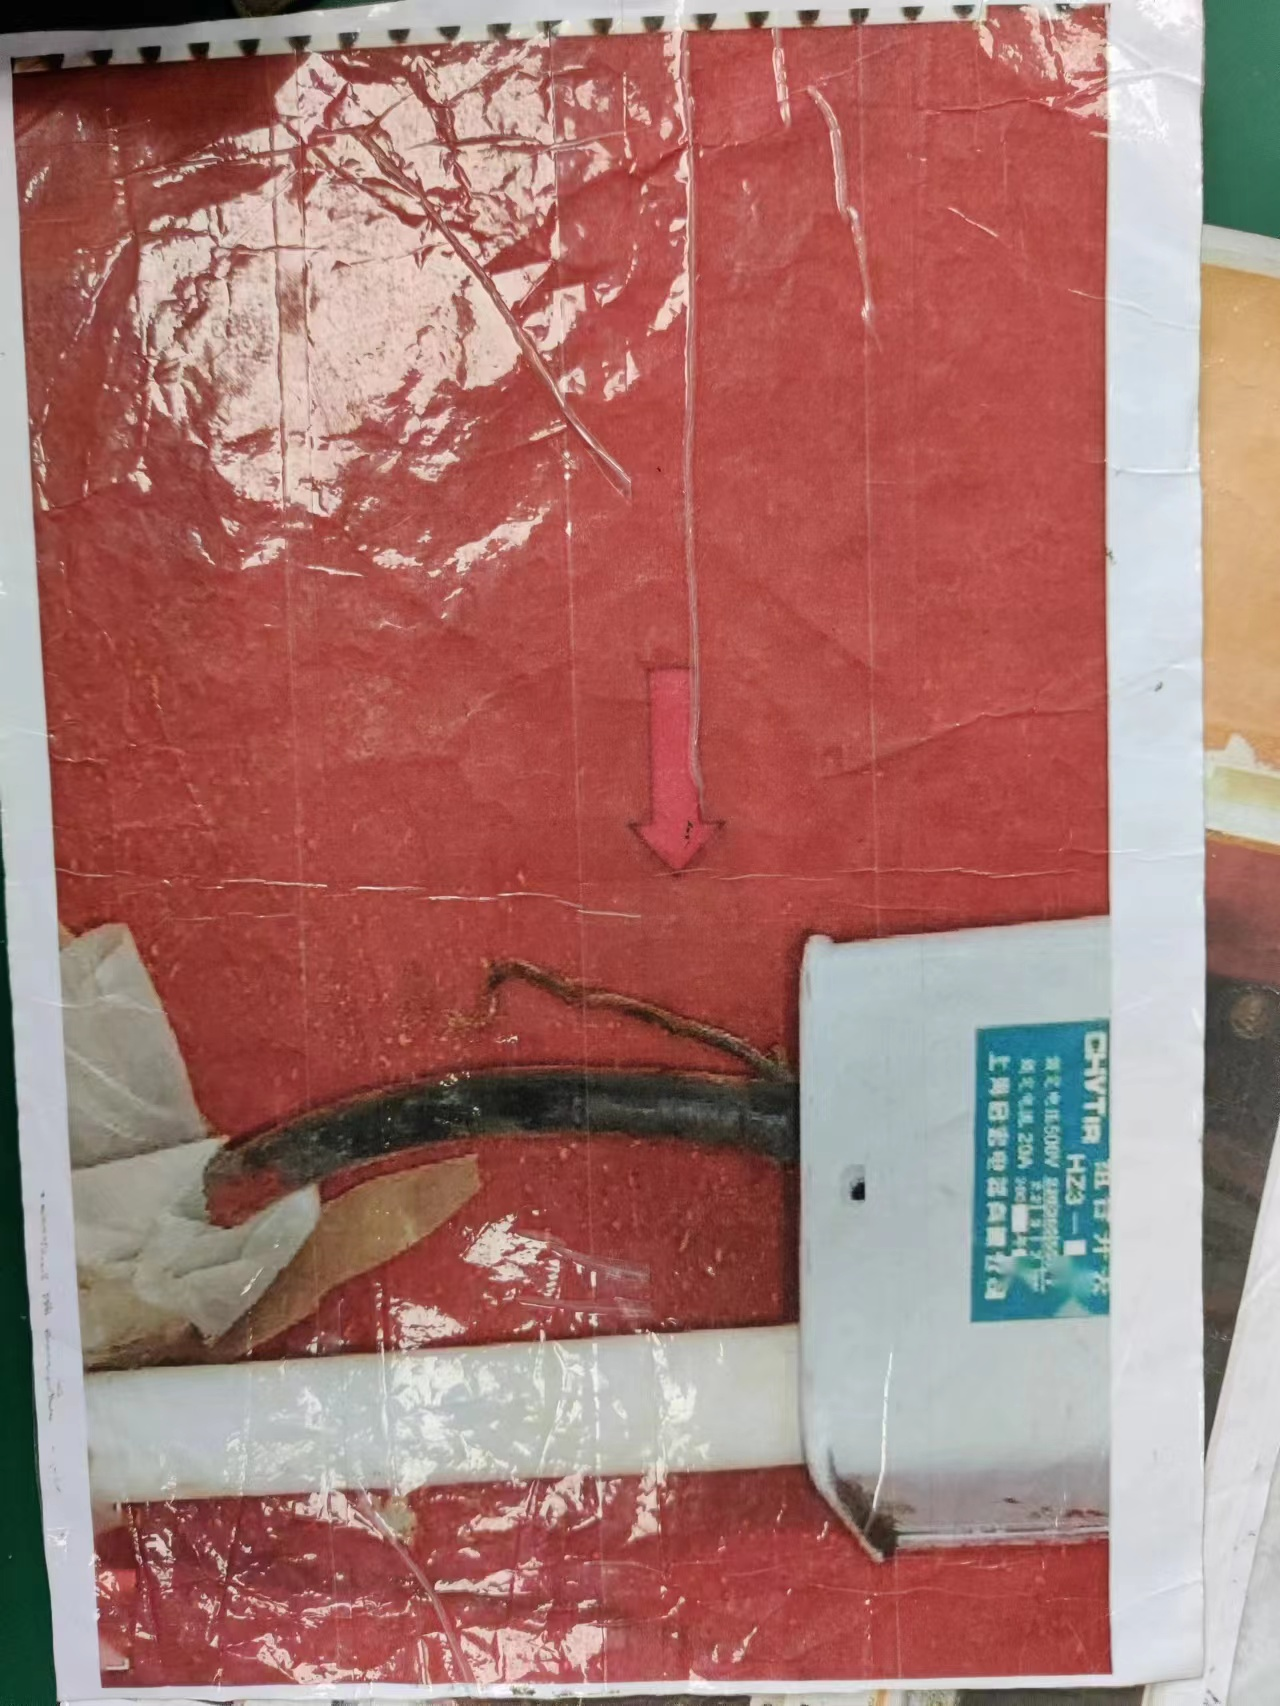
\includegraphics[width = 0.35\textwidth]{1}
    % \hfill
    \hspace*{1cm}
    % 
\includegraphics[width = 0.35\textwidth,trim = 500 200 300 400,clip,angle=0]{cover16}
    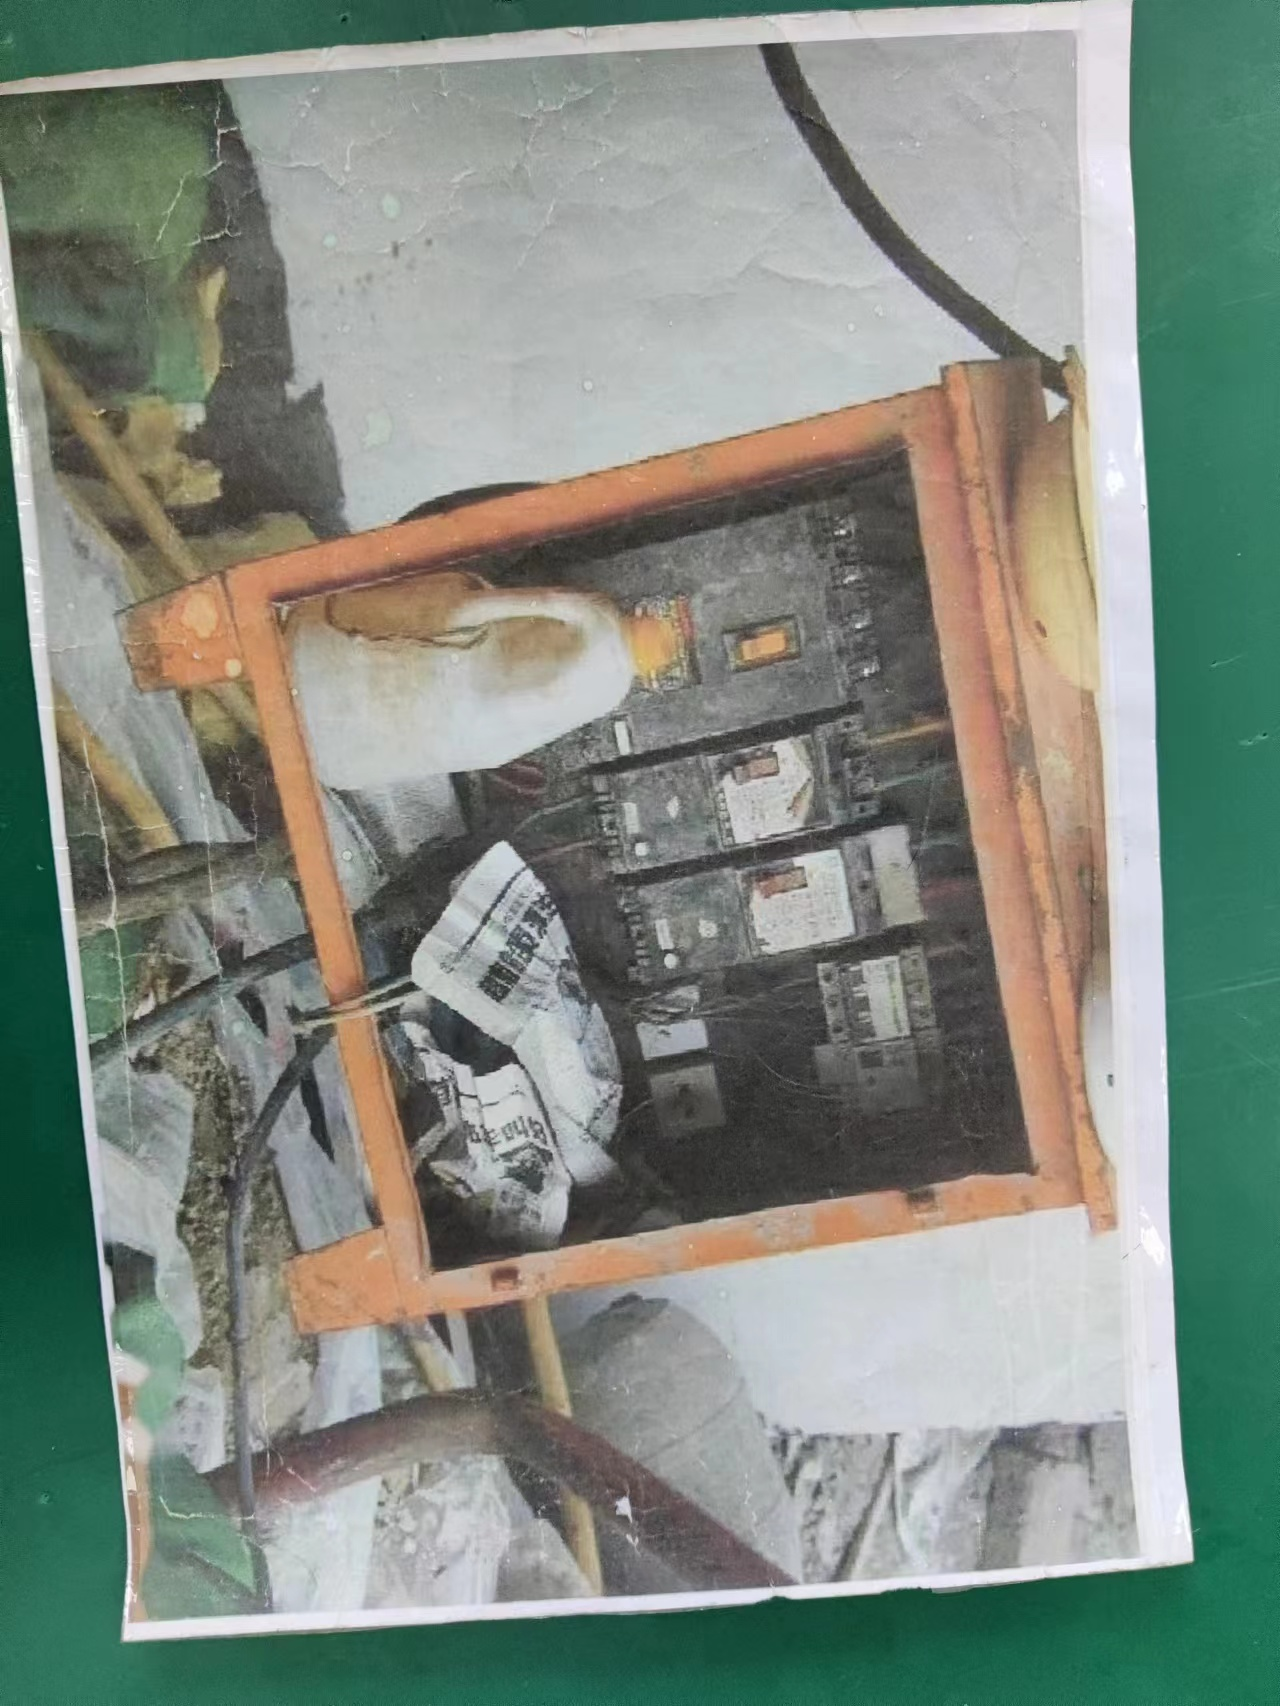
\includegraphics[width = 0.35\textwidth,angle=0]{3}
    \caption{有图有真相}
    \label{fig:myphoto}
\end{figure}


\section{一行两张图小标题}


\begin{figure}[!htbp]
    \centering
    \begin{minipage}[t]{0.45\textwidth}
        \centering
        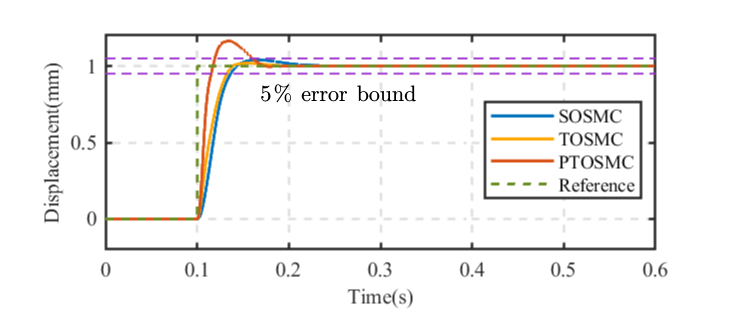
\includegraphics[width=\textwidth]{5-1} % 替换为你的图片文件名
        \caption{图像 1}
        \label{fig1a}
    \end{minipage}
    \begin{minipage}[t]{0.45\textwidth}
        \centering
        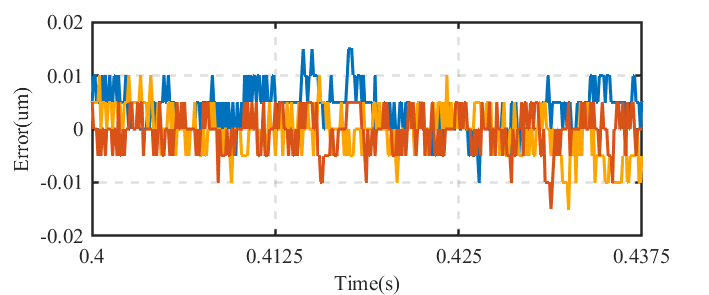
\includegraphics[width=\textwidth]{5-2} % 替换为你的图片文件名
        \caption{图像 2}
        \label{fig1b}
    \end{minipage}
    \caption{两个图像的并排显示}
    \label{fig1}
\end{figure}



\begin{figure}[!htbp]
    \centering
    \begin{subfigure}[b]{0.45\textwidth}
        \centering
        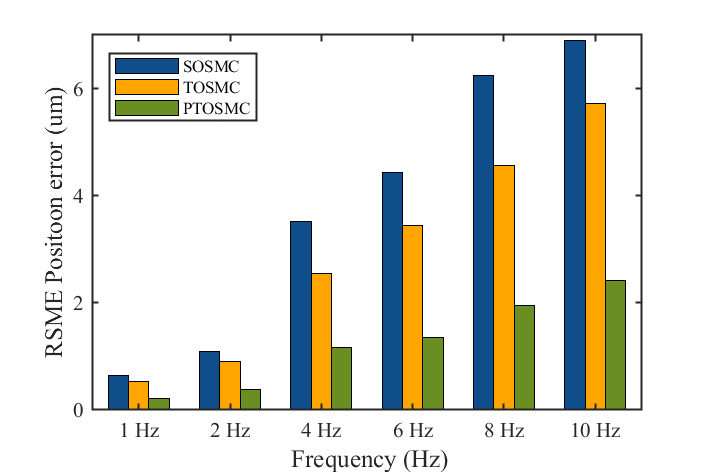
\includegraphics[width=\textwidth]{10} % 替换为你的图片文件名
        \caption{图像 1}
        \label{fig:sub1}
    \end{subfigure}
    \hspace*{1cm}
    \begin{subfigure}[b]{0.45\textwidth}
        \centering
        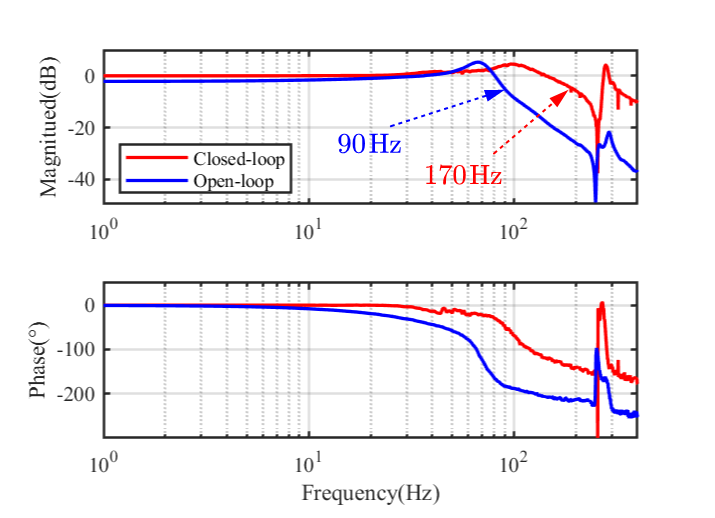
\includegraphics[width=\textwidth]{11} % 替换为你的图片文件名
        \caption{图像 2}
        \label{fig:sub2}
    \end{subfigure}
    \caption{两个图像的并排显示}
    \label{fig:main}
\end{figure}


%%%%%%%%%%%%%%%%%%%%%%%%%%%%%%%%%%%%%%%%%%%%%%%%%%%%%%%%%%%%%%%%%%%%%%%%%%%%%%%%%%%%%%%%%%%%%%%%%%%%%% 参考文献
    \printbibliography[heading=bibintoc, title=\ebibname]
%%%%%%%%%%%%%%%%%%%%%%%%%%%%%%%%%%%%%%%%%%%%%%%%%%%%%%%%%%%%%%%%%%%%%%%%%%%%%%%%%%%%%%%%%%%%%%%% 附录
    \appendix

    

% \appendix

\chapter{基本数学工具}


这是索引











\begin{table}[htb]
    \centering
        \begin{tabular}{ccc}
            \toprule
                 Header 1 & Header 2 & Header 3 \\
            \midrule
                Row 1    & Data 1   & Data 2   \\
                Row 2    & Data 3   & Data 4   \\
            \bottomrule
        \end{tabular}
\end{table}
    % 

% \appendix

\chapter{eee}


这是索引


qwdqw

dwqqw






\begin{table}[htb]
    \centering
        \begin{tabular}{ccc}
            \toprule
                 Header 1 & Header 2 & Header 3 \\
            \midrule
                Row 1    & Data 1   & Data 2   \\
                Row 2    & Data 3   & Data 4   \\
            \bottomrule
        \end{tabular}
\end{table}
\end{document}
